\chapter{Swing-Up Design}\label{sec:swing-upDesign}
In this chapter a swing-up controller is designed based on \cite{kjAastrom}. The pendulum is started at rest, $\theta = \pi$, angle convention is specified in \autoref{fig:mechanicalDrawing}. The idea of the swing-up controller is to increase the mechanical energy in the system until it matches that of the desired end state, which is the upright position at rest, that is, $\theta = 0$ and $\dot{\theta} = 0$. The minimum energy in the system is the starting position at rest, which is considered to be zero as mentioned in the \textit{Model} \autoref{sec:model}. So the target energy is $E_{\mathrm{eq}} = 2 m g l$, that is, the potential energy of the pendulum in the unstable equilibrium.

Consider the pendulum dynamics from \autoref{eq:energyDerivedDynamicEquation1},
\begin{flalign}
&& J \ddot{\theta} - m l \cos \theta \ddot{x}_c - m g l \sin \theta  &= 0 \ \ \ , &  \unit{N \cdot m}   \label{eq:pendulumDynamics}
\end{flalign}
where $J = m l^2$ is the inertia and the pendulum friction is assumed to be zero. This equation captures the behavior of the pendulum corresponding to some acceleration $\ddot{x}_c$ at the pivot point. This acceleration is viewed as the control input for now. The force needed to achieve this acceleration is considered in the end of the design. It is further convenient to describe the energy of the pendulum with the coordinate frame fixed at its pivot point, see \autoref{fig:fixedCooredinateSystem}.
%
\begin{figure}[H]
  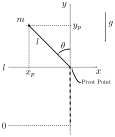
\includegraphics[width=.3\textwidth]{figures/fixedCooredinateSystem}
  \caption{The energy used in the swing-up controller is described using this convention, where the coordinate frame is fixed at the pivot point of the pendulum. The zero reference is placed as before s.t. all energies are positive.}
  \label{fig:fixedCooredinateSystem}
\end{figure}
%
From \autoref{fig:fixedCooredinateSystem}, the conversion from excessive to generalized coordinates is given by,
\begin{flalign}
&& x_p  &= -l \sin \theta   \ \ \ ,\ \ \ y_p = l(\cos \theta + 1)  \ \ \ ,\ \ \ \dot{x}_p = -l \cos \theta \dot{\theta}  \ \ \ ,\ \ \ \dot{y}_p = -l \sin \theta \dot{\theta}  \ \ \ . &&     \label{eq:cooredinateConvertFixed}
\end{flalign}
The mechanical energy in this coordinate frame is then,
\begin{flalign}
&& E_p &= m g y_p + \tfrac{1}{2} m \dot{x}_p^2 + \tfrac{1}{2} m \dot{y}_p^2  &  \unit{J}   \label{eq:pendulumEnergy1} \\
&& E_p &= m g l (\cos \theta +1) + \tfrac{1}{2} m (-l \cos \theta \dot{\theta})^2 + \tfrac{1}{2} m (-l \sin \theta \dot{\theta})^2  &  \unit{J}   \label{eq:pendulumEnergy2} \\
&& E_p &= m g l (\cos \theta +1) + \tfrac{1}{2} J (\cos^2 \theta  + \sin^2 \theta )\dot{\theta}^2  &  \unit{J}   \label{eq:pendulumEnergy3} \\
&& E_p &= \tfrac{1}{2} J \dot{\theta}^2 + m g l (\cos \theta +1) \ \ \ . &  \unit{J}   \label{eq:pendulumEnergy4}
\end{flalign}

\subsection{Energy Control}
A Lyapunov function candidate is proposed,
\begin{flalign}
&& V &= \tfrac{1}{2} E_\Delta ^2 \ \ \ ,  \hspace{5cm}  &&&  \label{eq:lyapunovCandidate} 
\end{flalign}
where $E_\Delta$ is the difference in energy in relation to the unstable equilibrium,
%
\begin{flalign}
&& E_\Delta &= E_p  - E_{\mathrm{eq}} &  \unit{J}   \label{eq:energyDelta1} \\
&& E_\Delta &= \tfrac{1}{2} J \dot{\theta}^2 + m g l (\cos \theta +1) - 2 m g l &  \unit{J}   \label{eq:energyDelta2} \\
&& E_\Delta &= \tfrac{1}{2} J \dot{\theta}^2 + m g l (\cos \theta -1)   \ \ \ .  & \unit{J} \label{eq:energyDelta3}
\end{flalign}
%
The derivative of $E_\Delta$ from \autoref{eq:energyDelta3} along the system \autoref{eq:pendulumDynamics} is found to,
\begin{flalign}
&& \dot{E}_\Delta &= J \dot{\theta} \ddot{\theta} - m g l \sin \theta \dot{\theta}  &&&   \label{eq:energyDeltaDerivative1} \\
&& \dot{E}_\Delta &= \dot{\theta} ( m l \cos \theta \ddot{x}_c + m g l \sin \theta )  - m g l \sin \theta \dot{\theta}    &&&   \label{eq:energyDeltaDerivative2} \\
&& \dot{E}_\Delta &=  m l \cos \theta \dot{\theta} \ddot{x}_c \ \ \ .   &&&   \label{eq:energyDeltaDerivative3}
\end{flalign}
%
The Lyapunov function candidate, \autoref{eq:lyapunovCandidate}, is continuously differentiable in the entire $\mathbb{R} ^2$ \fxnote{brush up on stability criteries}. Its derivative is evaluated to find a stabilizing controller,
%
\begin{flalign}
&& \dot{V} &= E_\Delta \dot{E}_\Delta   \hspace{3cm}  &&&  \label{eq:lyapunovDerivative1}  \\
&& \dot{V} &= E_\Delta m l \cos \theta \dot{\theta} \ddot{x}_c  \leq 0  \ \ \ .  \hspace{3cm}  &&&  \label{eq:lyapunovDerivative2} 
\end{flalign}
%
The acceleration, $\ddot{x}_c$, is then designed to satisfy the stability criterion in \autoref{eq:lyapunovDerivative2},
\begin{flalign}
&& \dot{V} &= m l E_\Delta \cos \theta \dot{\theta} (-E_\Delta \cos \theta \dot{\theta})     \hspace{2cm}  &&&  \label{eq:lyapunovDerivativeControlled1} \\
&& \dot{V} &= -m l (E_\Delta \cos \theta \dot{\theta})^2  \leq 0  \ \ \ ,  \hspace{2cm}  &&&  \label{eq:lyapunovDerivativeControlled2} 
\end{flalign}
further a tuning parameter, $k>0$, is introduced such that the control law for acceleration of the pivot point is,
\begin{flalign}
&& \ddot{x}_c &= -k E_\Delta \cos \theta \dot{\theta}  \ \ \ .  \hspace{4cm}  &&&  \label{eq:accControlLaw} 
\end{flalign}
If this control law is started at zero angular velocity, $\dot{\theta} = 0$, in a stable equilibrium, the computed control is maintained at zero and the pendulum never swings up. So for this control law to work, the pendulum must be started slightly away from a stable equilibrium. The control is also zero when $\cos\theta = 0$, however, when this occurs the system is not in a stable equilibrium and the zero value of $\ddot{x}_c$ is therefore not maintained in these cases.

An extra step is needed to apply this control strategy. So far the control output is an acceleration, $\ddot{x}_c$, at the pivot point. It is possible to input the desired acceleration, $\ddot{x}_c$, into the second dynamic equation, \autoref{eq:energyDerivedDynamicEquation1}, and solve for the force needed to achieve this acceleration,
%
\begin{flalign}
  && u &=  ( M + m )\ddot{x}_c + m l \sin x_1 x_3^2 - m l \cos x_1 \dot{x}_3  \ \ \ , &   \unit{N}
  \label{eq:forceDynamics}
\end{flalign}
%
where the cart friction coefficients are set to zero again.\\
To calculate the force from this expression, \autoref{eq:forceDynamics}, it is also necessary to know the angular acceleration of the pendulum, $\dot{x}_3$, which can be solved for in the system dynamics, \autoref{eq:nonlinearStateSpace}, inserting known states and control input applied in the previous step,
%
\begin{flalign}
  &&
    \begin{bmatrix}
      \dot{x}_3  \\
      \dot{x}_4
    \end{bmatrix}
    &=
    \begin{bmatrix}
      m l^2           & -m l \cos x_1  \\
      -m l \cos x_1   & M + m
    \end{bmatrix}^{-1}
    \begin{bmatrix}
      - b_{p,v} x_3 - \tanh(\text{k}_\text{tanh}x_3) b_{p,c} + m g l \sin x_1 \\
      u_{last} - m l \sin x_1 x_3^2
    \end{bmatrix}
     \ \ \ ,  &&
  \label{eq:nonlinearStateSpaceQdotDot}
\end{flalign}
%
where $u_{last}$ is the force applied in the previous step.\\
From \autoref{eq:nonlinearStateSpaceQdotDot} the approximated angular acceleration is then,
\begin{flalign}
  && \dot{x}_3 &= \frac{ ( M + m )(- b_{p,v} x_3 - \tanh(\text{k}_\text{tanh}x_3) b_{p,c} + m g l \sin x_1) }{ l^2 m ( M + m - m \cos^2x_1 ) }
                    + \frac{ \cos x_1 (u_{last} - m l \sin x_1 x_3^2) }{ l ( M + m - m \cos x_1^2 ) }
  \ \ \ .  &&
  \label{eq:thetaDotDotApprox}
\end{flalign}
%
Inserting \autoref{eq:thetaDotDotApprox} into \autoref{eq:forceDynamics} results in the control input, $u$, necessary to achieve the desired acceleration, $\ddot{x}_c$, at the pivot point. This method is used for all swing-up controllers, so to avoid excessive notation the proceeding energy control laws are derived with $\ddot{x}_c$ as the control parameter.

All simulations are performed using the nonlinear state space representation in \autoref{eq:nonlinearStateSpace} and the matlab ODE45 solver with relative tolerance of \SI{1e-7}{}. Initializing the angle, $\theta$, at $\pi-0.1$ to avoid zero control output as discussed, the energy difference struggles to reach its reference at zero, see \autoref{fig:Edelta_1_noConX}.
%
\begin{figure}[H]
  \includegraphics[width=.5\textwidth]{figures/Edelta_1_noConX}
  \caption{Edelta1noConX}
  \label{fig:Edelta_1_noConX}
\end{figure}
%
The pendulum also falls short of reaching the heteroclinic orbit, see \autoref{fig:phase_1_noConX}. \fxnote{include small section on heteroclinic orbit}
Some energy is lost to friction in the pendulum. The cart however is considered to be frictionless in both design and simulation for now.\fxnote{section on friction compensation}
\begin{figure}[H]
  \includegraphics[width=.5\textwidth]{figures/phase_1_noConX}
  \caption{phase1noConX}
  \label{fig:phase_1_noConX}
\end{figure}
%
However, as the energy of the pendulum is not affected by the position or velocity of the cart, this control law, \autoref{eq:accControlLaw}, is not concerned with controlling these. This becomes a problem in the physical setup as it has a rail length of one meter. A traced animation is used to demonstrate this problem in \autoref{fig:ani_1_noConX}.
\begin{figure}[H]
  \includegraphics[width=.7\textwidth]{figures/ani_1_noConX}
  \caption{ani1noConX}
  \label{fig:ani_1_noConX}
\end{figure}
%
An other issue is the actuation which is limited in the real system by the maximum allowed continuous current, see \autoref{table:systemParameters}. By tuning the parameter $k$ in \autoref{eq:accControlLaw}, better performance can be obtained, however at the cost of excessive actuation.
%
\begin{figure}[H]
  \includegraphics[width=.52\textwidth]{figures/ia_1_noConX}
  \caption{ia1noConX}
  \label{fig:ia_1_noConX}
\end{figure}
%
For these graphs $k=1.3$ to keep the motor current at acceptable levels. The motor current is shown in \autoref{fig:ia_1_noConX} where the rolling RMS of $i_a$ is used to approximate the continuous current load on the motor.

%\begin{figure}[H]
%  \includegraphics[width=.6\textwidth]{figures/x_1_noConX}
%  \caption{x1noConX}
%  \label{fig:x_1_noConX}
%\end{figure}
%\begin{figure}[H]
%  \includegraphics[width=.6\textwidth]{figures/xDot_1_noConX}
%  \caption{xDot1noConX}
%  \label{fig:xDot_1_noConX}
%\end{figure}
%\begin{figure}[H]
%  \includegraphics[width=.6\textwidth]{figures/xDotDot_1_noConX}
%  \caption{xDotDot1noConX}
%  \label{fig:xDotDot_1_noConX}
%\end{figure}
%\begin{figure}[H]
%  \includegraphics[width=.6\textwidth]{figures/theta_1_noConX}
%  \caption{theta1noConX}
%  \label{fig:theta_1_noConX}
%\end{figure}
%\begin{figure}[H]
%  \includegraphics[width=.6\textwidth]{figures/thetaDot_1_noConX}
%  \caption{thetaDot1noConX}
%  \label{fig:thetaDot_1_noConX}
%\end{figure}
%\begin{figure}[H]
%  \includegraphics[width=.6\textwidth]{figures/thetaDotDot_1_noConX}
%  \caption{thetaDotDot1noConX}
%  \label{fig:thetaDotDot_1_noConX}
%\end{figure}


\subsection{Sign-Based Energy Control}


\begin{figure}[H]
  \includegraphics[width=.5\textwidth]{figures/Edelta_2_noConX}
  \caption{Edelta2noConX}
  \label{fig:Edelta_2_noConX}
\end{figure}
%
\begin{figure}[H]
  \includegraphics[width=.5\textwidth]{figures/phase_2_noConX}
  \caption{phase2noConX}
  \label{fig:phase_2_noConX}
\end{figure}
%
\begin{figure}[H]
  \includegraphics[width=1\textwidth]{figures/ani_2_noConX}
  \caption{ani2noConX}
  \label{fig:ani_2_noConX}
\end{figure}
%
\begin{figure}[H]
  \includegraphics[width=.52\textwidth]{figures/ia_2_noConX}
  \caption{ia2noConX}
  \label{fig:ia_2_noConX}
\end{figure}


%\begin{figure}[H]
%  \includegraphics[width=.6\textwidth]{figures/x_2_noConX}
%  \caption{x2noConX}
%  \label{fig:x_2_noConX}
%\end{figure}
%\begin{figure}[H]
%  \includegraphics[width=.6\textwidth]{figures/xDot_2_noConX}
%  \caption{xDot2noConX}
%  \label{fig:xDot_2_noConX}
%\end{figure}
%\begin{figure}[H]
%  \includegraphics[width=.6\textwidth]{figures/xDotDot_2_noConX}
%  \caption{xDotDot2noConX}
%  \label{fig:xDotDot_2_noConX}
%\end{figure}
%\begin{figure}[H]
%  \includegraphics[width=.6\textwidth]{figures/theta_2_noConX}
%  \caption{theta2noConX}
%  \label{fig:theta_2_noConX}
%\end{figure}
%\begin{figure}[H]
%  \includegraphics[width=.6\textwidth]{figures/thetaDot_2_noConX}
%  \caption{thetaDot2noConX}
%  \label{fig:thetaDot_2_noConX}
%\end{figure}
%\begin{figure}[H]
%  \includegraphics[width=.6\textwidth]{figures/thetaDotDot_2_noConX}
%  \caption{thetaDotDot2noConX}
%  \label{fig:thetaDotDot_2_noConX}
%\end{figure}

\subsection{Sat-Based Energy Control}

%\begin{figure}[H]
%  \includegraphics[width=.5\textwidth]{figures/Edelta_2_noConX}
%  \caption{Edelta1noConX}
%  \label{fig:Edelta_2_noConX}
%\end{figure}
%%
%\begin{figure}[H]
%  \includegraphics[width=.5\textwidth]{figures/phase_2_noConX}
%  \caption{phase1noConX}
%  \label{fig:phase_2_noConX}
%\end{figure}
%%
%\begin{figure}[H]
%  \includegraphics[width=.7\textwidth]{figures/ani_2_noConX}
%  \caption{ani1noConX}
%  \label{fig:ani_2_noConX}
%\end{figure}
%%
%\begin{figure}[H]
%  \includegraphics[width=.52\textwidth]{figures/ia_2_noConX}
%  \caption{ia1noConX}
%  \label{fig:ia_2_noConX}
%\end{figure}
%
%
%\begin{figure}[H]
%  \includegraphics[width=.6\textwidth]{figures/x_2_noConX}
%  \caption{x1noConX}
%  \label{fig:x_2_noConX}
%\end{figure}
%\begin{figure}[H]
%  \includegraphics[width=.6\textwidth]{figures/xDot_2_noConX}
%  \caption{xDot1noConX}
%  \label{fig:xDot_2_noConX}
%\end{figure}
%\begin{figure}[H]
%  \includegraphics[width=.6\textwidth]{figures/xDotDot_2_noConX}
%  \caption{xDotDot1noConX}
%  \label{fig:xDotDot_2_noConX}
%\end{figure}
%\begin{figure}[H]
%  \includegraphics[width=.6\textwidth]{figures/theta_2_noConX}
%  \caption{theta1noConX}
%  \label{fig:theta_2_noConX}
%\end{figure}
%\begin{figure}[H]
%  \includegraphics[width=.6\textwidth]{figures/thetaDot_2_noConX}
%  \caption{thetaDot1noConX}
%  \label{fig:thetaDot_2_noConX}
%\end{figure}
%\begin{figure}[H]
%  \includegraphics[width=.6\textwidth]{figures/thetaDotDot_2_noConX}
%  \caption{thetaDotDot1noConX}
%  \label{fig:thetaDotDot_2_noConX}
%\end{figure}











